\documentclass[]{article}
\usepackage{hyperref}
\hypersetup{colorlinks=true}
\usepackage{graphicx}

\begin{document}

\title{Title}
\author{Author}
\date{Today}
\maketitle

\section{Current Industry State}

While the current industry has attempted to use Computer Vision and Image Processing for Quality Assurance, attempts have often been expensive and cumbersome. Take the example of  \href{http://www.avt-inc.com/?catid=\%7B757EF709-E4DF-4C16-A2E7-5F7866D891AC\%7D}{AVT Inc, Israel} that sells high quality instruments that use spectral imaging techniques to look for defects in fabrics. While these techniques may be useful and necessary in fabrics for aeronautical and structural purposes, this appears to be plain and simple overkill for garment fabrics. Also, research in this field has more or less remained stagnant after 2006, leaving the algorithms that run these processes fairly inefficient.

\section{Literature Review}

We have reviewed several findings and research papers(our internet history from yesterday should be a testament to that). Here we will discuss the standard methods used by various researchers across the world.
\begin{itemize}
\item One of the most popular techniques is edge detection using Gabor filters. Its impulse response is defined by a sinusoidal wave (a plane wave for 2D Gabor filters) multiplied by a Gaussian function. A set of Gabor filters with different frequencies and orientations may be helpful for extracting useful features from an image. Gabor filters have been widely used in pattern analysis applications. In the research paper by \href{http://hub.hku.hk/bitstream/10722/46561/1/131190.pdf}{HKU}, this technique is used extensively for plain, twill and denim fabrics.  
\begin{center}
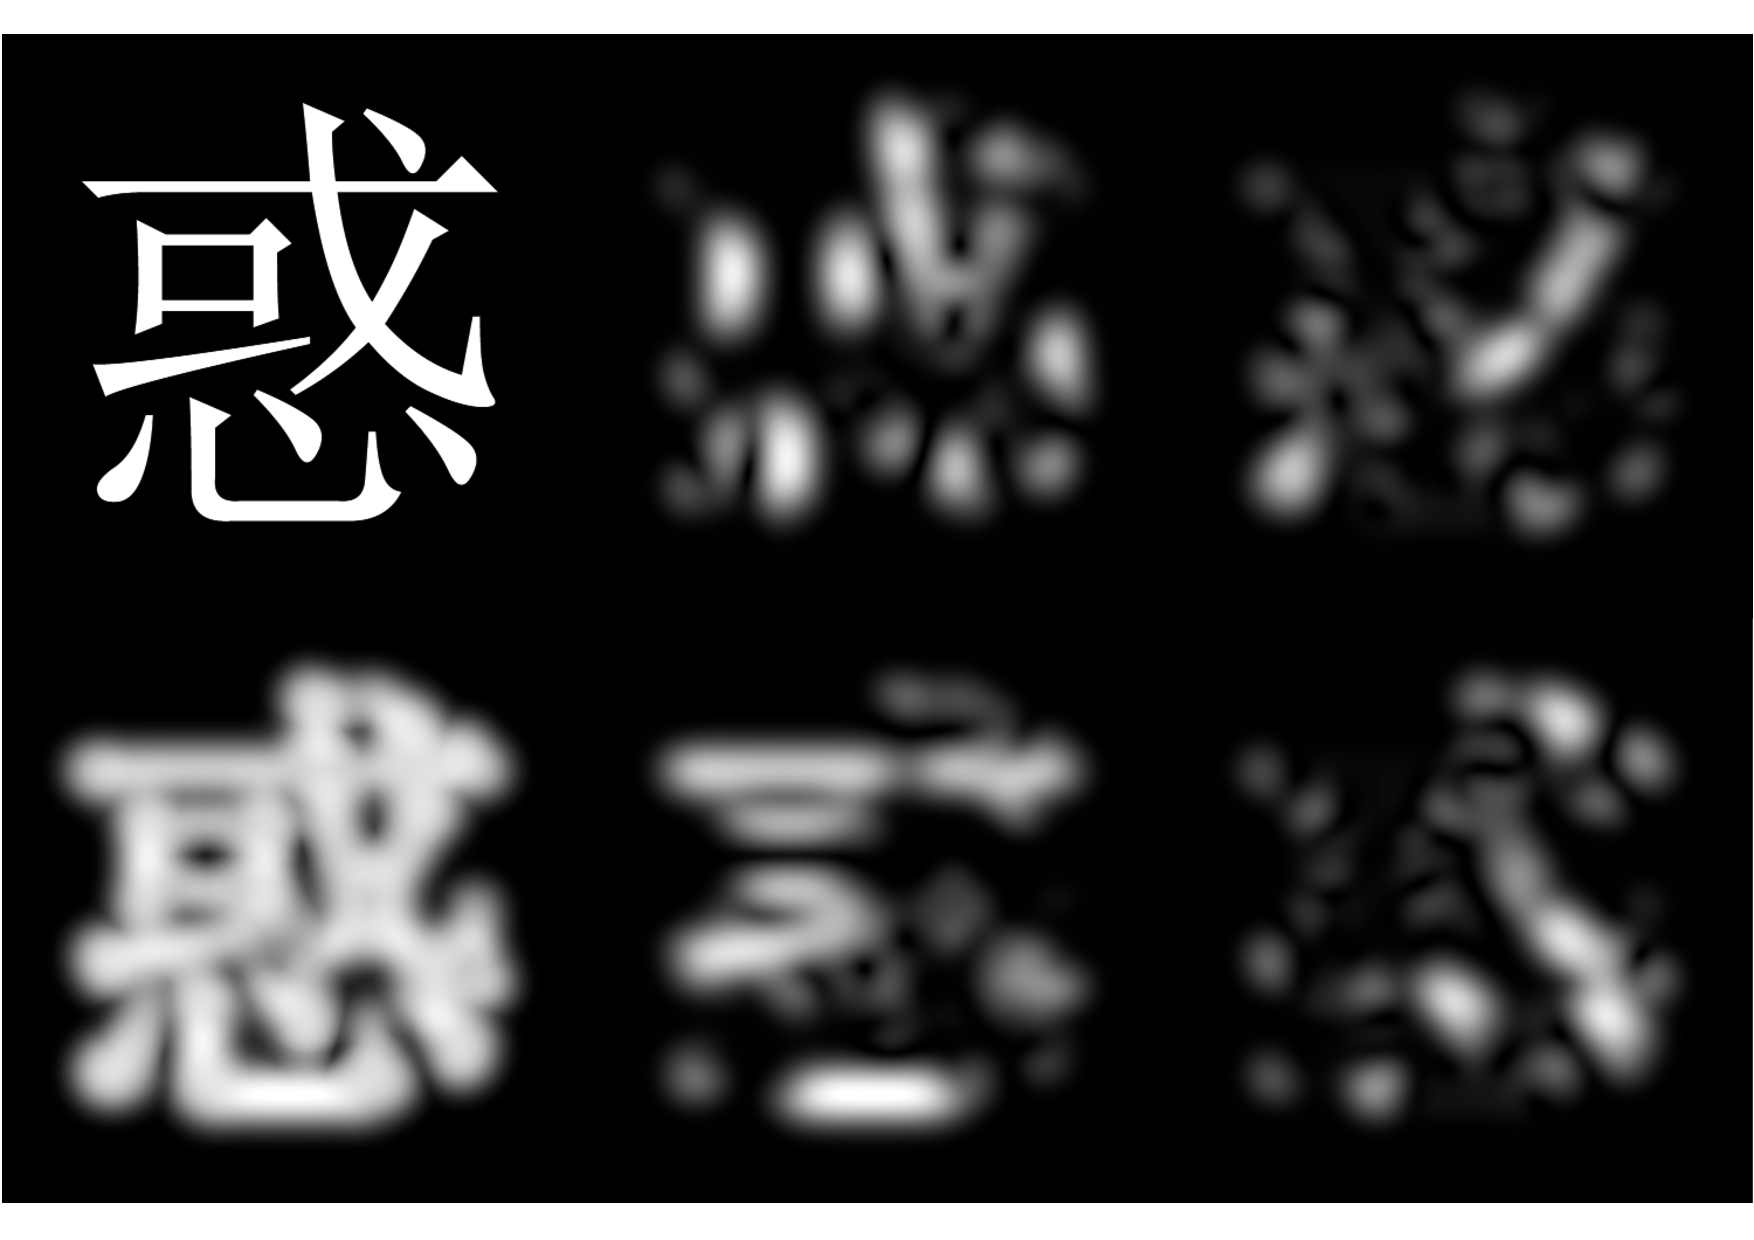
\includegraphics[width=4in]{/Users/robinmalhotra2/Developer/Mini-Project/Gabor-ocr.pdf}

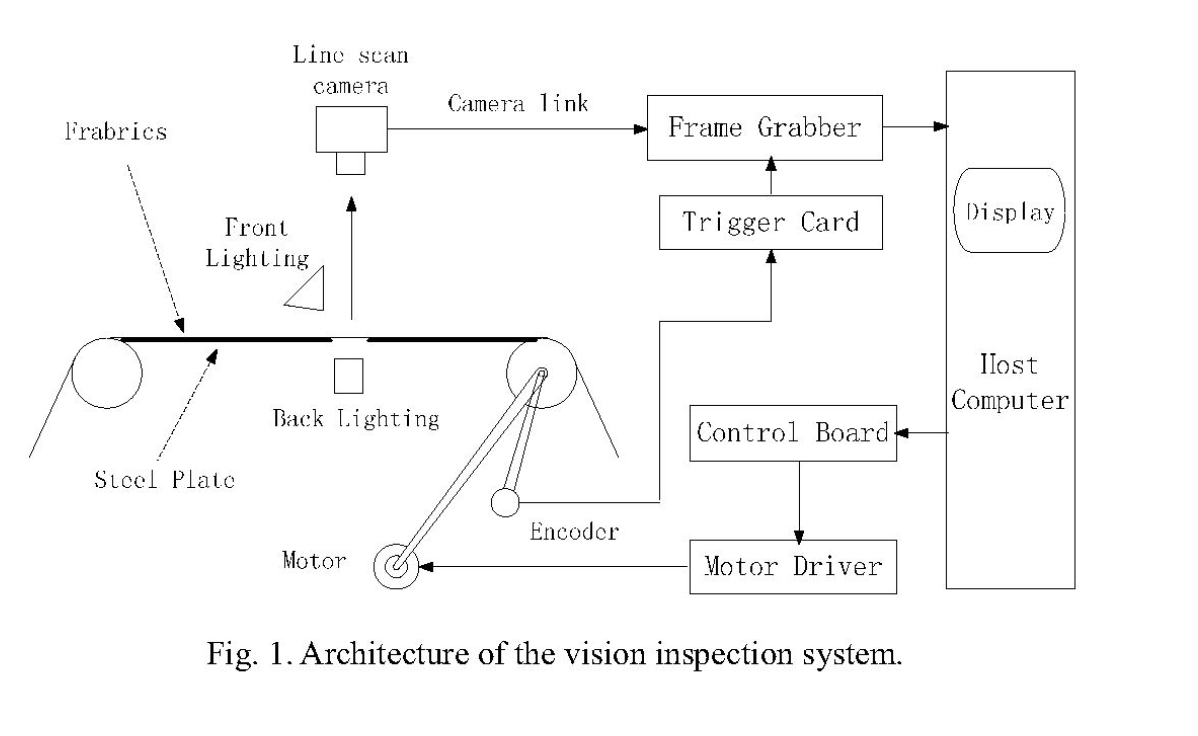
\includegraphics[width=4in]{/Users/robinmalhotra2/Developer/Mini-Project/Plan}



\end{center}
\textbf{Filter selection and detection Algorithm:}
\begin{enumerate}
\item $g_c(x,y)=e^{-\frac{1}{2} \big[ \big(\frac{ x^{'}}{\sigma_x} \big)^2 +  \big(\frac{ y^{'}}{\lambda \sigma_x} \big)^2 \big]} \cos \big[2\pi \mu_0 x^{'}\big]$
where   $x^{'}$ and  $y^{'}$ are the rotated transformed values of the x and y coordinates.$ \mu_0$ is the frequency of a sinusoidal wave along the x axis and $\lambda$ is the ratio between the variances in the y and x directions.
\item $E=\sum_{x,y}\big[ IM(x,y)-w^{i}g_{e}^{i}(x,y) \big]^{2}$
where g is the gabor function in x,y 
 \item By minimising the above function, we create an optimal solution from a set of 7 real filters(by changing various parameters). Generally the size of defects is greater than a yarn, the filtering results with finer resolutions than a yarn contribute very little for segmenting defects.
\item $O_f=\sum_{i=1}^{J} a^i f^i \big( f^i= IM*g_e^i ; a^i=\alpha^i / \sum_{k=1}^{J} \alpha^k \big)$
Note that the image data here is the fourier convolution.
\item Finally,the final binary segmentation result of a fabric is obtained by thresholding output from  the median filtering step.
\begin{center}
 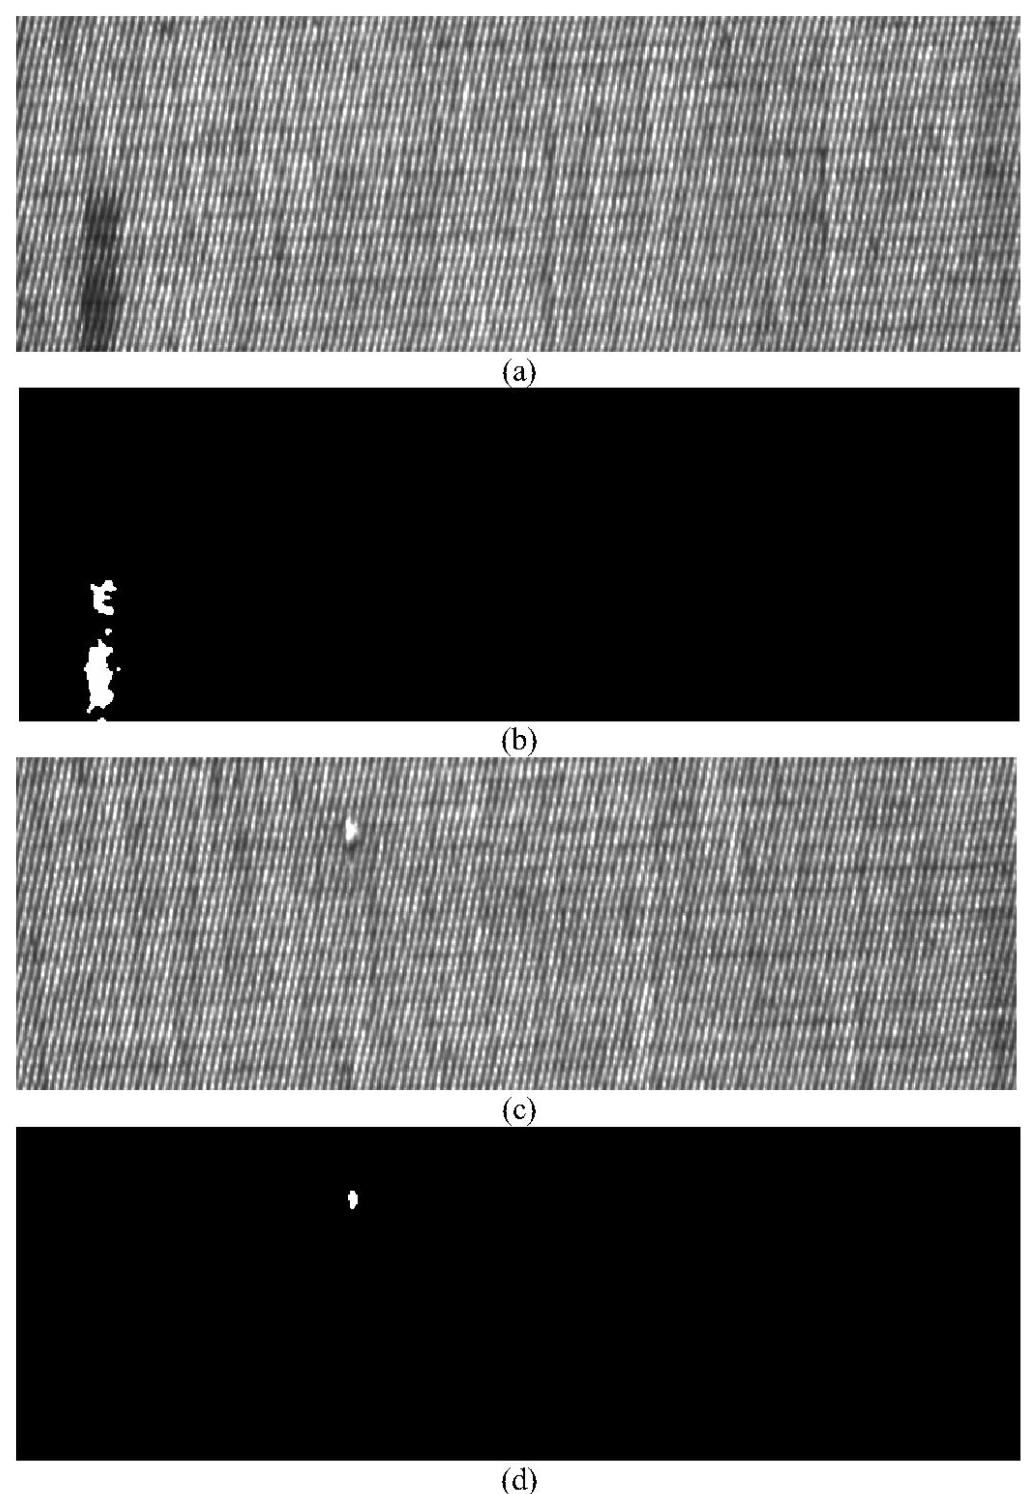
\includegraphics[width=4in]{/Users/robinmalhotra2/Developer/Mini-Project/flowChart.png}
System Performance
\end{center}
\end{enumerate}

\item \textbf{Defect detection using bi-level thresholding:}Another method for defect detection is bilevel thresholding. This involves scanning across the width  of the grayscale image. A histogram is plotted to produce 2 sets of pixels: $G_1$ consisting of pixels with grey level $T\geq T_1$ and $G_2$ with $T\geq T_2$. We will then find the average value $\mu_1$ and $\mu_2$  

\item Another method is Fractal Dimensions. This basically tries to detect an irregular geometric object with an infinite nesting of structure at all scales. The localization accuracy of these detected defects is very poor and have high false alarm. For more information, refer \href{http://www.vanderbilt.edu/AnS/psychology/cogsci/chaos/workshop/Fractals.html}{here}



\end{itemize} 



\end{document}